\documentclass[11pt]{SelfArx}

\PassOptionsToPackage{usenames,dvipsnames}{xcolor}
%!TEX root = ./2017_NSF_proposal.tex
\AtBeginDocument{%
  \addtolength\abovedisplayskip{-0.5\baselineskip}%
  \addtolength\belowdisplayskip{-0.5\baselineskip}%
%  \addtolength\abovedisplayshortskip{-0.5\baselineskip}%
%  \addtolength\belowdisplayshortskip{-0.5\baselineskip}%
}



\usepackage{fec}
\usepackage[sort&compress]{natbib}
 \usepackage{comment}
\usepackage{graphicx}
\usepackage{multirow}
\usepackage{multicol}

% \RequirePackage{algorithmic,algorithm}




\newcommand{\tr}{\textrm{tr}}

\newcommand{\inTR}[1]{}
\newcommand{\setN}{N}

\usepackage{algorithm}
% \usepackage{algorithmic}
\usepackage{algpseudocode}

\usepackage[colorinlistoftodos,bordercolor=orange,backgroundcolor=orange!20,linecolor=orange,textsize=scriptsize]{todonotes}


%\usepackage[disable]{todonotes}



%\JournalInfo{\today} % Journal information
%\Archive{XXXX} % Additional notes (e.g. copyright, DOI, review/research article)


%\Authors{}
%\Keywords{} % Keywords - if you don't want any simply remove all the text between the curly brackets
\newcommand{\keywordname}{Keywords} % Defines the keywords heading name
%\Abstract{}


%\usepackage{subfigure}
%\usepackage{subfig}
\usepackage{enumitem}

\usepackage{epsfig}
\usepackage{color}
\usepackage{boxedminipage}
\usepackage{amsfonts}
\usepackage{amsmath}
\usepackage{url}

\usepackage{epstopdf}
\usepackage{enumitem}
\usepackage{natbib}
\usepackage{pdfpages}
\newcommand{\note}[1]{{\small \color{red} \it #1}}



\setlength{\bibsep}{0pt plus 0.3ex}
\setlength{\columnsep}{0.55cm} % Distance between the two columns of text
\setlength{\fboxrule}{0.75pt} % Width of the border around the abstract


%\usepackage{fontspec}
%\setmainfont{Arial}

 \newtheorem{theorem}{Theorem}
 \newtheorem{lemma}{Lemma}
% \newtheorem{propres}{Proposed Research}
%\newtheorem{propres}{Research Topic}
\newtheorem{propres}{Framework}

%---------------------------------------------------------------------------------------
%   COLORS
%----------------------------------------------------------------------------------------
\definecolor{color1}{HTML}{81071c} %   0,0,90  Color of the article title and sections
\definecolor{color2}{RGB}{0.972549,0.8352941, 0.5137255} % Color of the boxes behind the abstract and headings
\definecolor{light-gray}{gray}{0.1}
\color{light-gray}


%----------------------------------------------------------------------------------------
%   ABSTRACT
%----------------------------------------------------------------------------------------



\usepackage{epsfig}
\usepackage{epstopdf}

%----------------------------------------------------------------------------------------
%   HYPERLINKS
%----------------------------------------------------------------------------------------
% \usepackage{hyperref} % Required for hyperlinks

\newcommand\tagthis{\addtocounter{equation}{1}\tag{\theequation}}


\usepackage{amsmath}
\DeclareMathOperator{\Rand}{Rand}
\DeclareMathOperator{\support}{support}



% revision and comment
\usepackage[normalem]{ulem}
\usepackage[dvipsnames]{xcolor}
\newcommand{\del}[1]{{\ignorespaces \color{red} \sout{#1}}}
\newcommand{\add}[1]{{\color{blue} {#1}}}
\newcommand{\rewrite}[1]{{\color{SeaGreen} {#1}}}
\newcommand{\tored}[1]{{\color{red} {#1}}}



                       % such that
\newcommand{\ve}[2]{\left\langle #1 ,  #2 \right\rangle}    % inner product
\newcommand{\eqdef}{:=}
                    % set of real numbers
\newcommand{\Prob}{\mathbb{P}}                   % probability
                       % expectation

%\newcommand{\U}{U}
\newcommand{\argmin}{argmin}

\newcommand{\R}{ {\bf R}}
\newcommand{\Var}{\mathbf{Var}}
\newcommand{\hatZ}{\hat Z}
\newcommand{\hatS}{\hat S}
\newcommand{\calG}{G}
\newcommand{\calT}{\mathcal{T}}
\newcommand{\calF}{\mathcal{F}}
\newcommand{\Lip}{\mathcal{L}}
\newcommand{\calH}{\mathcal{H}_\beta}
\newcommand{\calHMINI}{\mathcal{C}}

\newcommand{\calS}{\mathcal{S}}
\newcommand{\calJ}{\mathcal{J}}
\newcommand{\x}{ {x}}
\newcommand{\y}{ {\bf y}}
\newcommand{\z}{ {\bf z}}
\newcommand{\vv}{ {\bf v}}
\newcommand{\wv}{ {\bf w}}
\newcommand{\av}{ {\bf \alpha}}
\newcommand{\bv}{ {\bf \alpha}}
\newcommand{\V}{ {\bf v}}
\newcommand{\T}{ {\bf T}}
\newcommand{\X}{ {\bf X}}

\newcommand{\0}{ {\bf 0}}
\newcommand{\alf}{ {\boldsymbol \alpha}}
\newcommand{\vchi}{ {\boldsymbol \chi}}

\newcommand{\vu}{{\bf u}}
\newcommand{\vdelta}{{\boldsymbol \delta} }
\newcommand{\w}{  {\bf w}}
\newcommand{\vt}{  {\bf t}}
\newcommand{\va}{  {\bf a}}

\newcommand{\f}{f}
\newcommand{\YY}{\varphi}
\newcommand{\K}{K}
\newcommand{\sK}{\mathcal{K}}
\newcommand{\J}{J}
\newcommand{\sJ}{\mathcal{J}}

\newcommand{\calO}{\mathcal{O}}
\newcommand{\vsubset}[2]{#1_{[#2]}}
\newcommand{\Srv}{\hat{S}}
\newcommand{\oo}{|J \cap \Srv_j|}

\newcommand{\vc}[2]{#1^{(#2)}}                   % coordinate of a vector
\newcommand{\cor}[2]{{{#1}_{#2}}}                   % coordinate of a vector
\newcommand{\corit}[3]{{#1}_{#2}^{(#3)}}                   % coordinate of a vector
\newcommand{\ncs}[2]{\|#1\|^2_{(#2)}}
\newcommand{\nbp}[2]{\|#1\|_{(#2)}}              % norm block primal
\newcommand{\nbd}[2]{\|#1\|_{(#2)}^*}            % norm block dual
\newcommand{\Rw}[2]{\mathcal R_{#1}(#2)}
\newcommand{\Rws}[2]{\mathcal R^2_{#1}(#2)}
        % Cardinality

\newcommand{\pnote}[1]{{  \color{red} [[ #1 -- Peter ]] }}
\newcommand{\natinote}[1]{{  \color{blue} [[ #1 -- Nati ]] }}
\newcommand{\takinote}[1]{{  \color{yellow} [[ #1 -- Martin ]] }}
\newcommand{\avnote}[1]{{  \color{green} [[ #1 -- Avleen ]] }}
\newcommand{\removed}[1]{}
\newcommand{\norm}[1]{\left\lVert{#1}\right\rVert}
\newcommand{\hingeloss}{\ell}
\newcommand{\hinge}[1]{\hingeloss ( #1 )}
\newcommand{\trans}{{\top}}
\newcommand{\calA}{\mathcal{A}}
\newcommand{\bP}{\mathcal{P}}
\newcommand{\bD}{\mathcal{D}}
\newcommand{\bH}{\mathcal{H}}
\newcommand{\sizeJ}{\omega}
\newcommand{\Gg}{\mathcal{G}^{\sigma'}}


\newcommand{\newstuff}[1]{{\color{red}#1}}
\newcommand{\cocoa}{\textsc{CoCoA}}
\newcommand{\cocoap}{\textsc{CoCoA$\!^{\bf \textbf{\footnotesize+}}$}}
\newcommand{\localalgname}{\textsc{LocalSolver}\xspace}
\newcommand{\localSDCA}{\textsc{LocalSDCA}\xspace}
\newcommand{\setn}{[n]}
\newcommand{\Exp}{\mathbb{E}}                      % expectation


\usepackage{caption}
\usepackage{subcaption}
%----------------------------------------------------------------------------------------
%   HYPERLINKS
%----------------------------------------------------------------------------------------
\usepackage{hyperref} % Required for hyperlinks
\hypersetup{colorlinks,breaklinks=true,urlcolor=color2,citecolor=color1,linkcolor=color1,bookmarksopen=false,pdftitle={Title},pdfauthor={Author}}
\usepackage{algorithm}
\usepackage{wrapfig}
\usepackage{hyperref}
\hypersetup{colorlinks,urlcolor=blue}


\begin{document}

\pagestyle{plain}

\begin{center}
{
\color{color1}
\bf \large
%Distributed Second-Order Algorithms for Large-Scale Machine Learning
  Facilities, Equipment, and Other Resources
 }
%
%
 \end{center}

\section*{Workshop Facilities}

\subsection*{Workshop Facilities at Lehigh}
Lehigh has numerous spaces that can accommodate workshops.  The \href{https://lehighmountaintop.wordpress.com/learn-more/}{Mountaintop Campus} houses several such spaces that have been used by the PIs and others for one-day events and multiple-day workshops. 

\subsection*{Workshop Facilities at I-DISC}
The \textbf{co-PI He} and \textbf{SP Agar, SP Takac} are are members of the \href{https://idisc.lehigh.edu/}{Institute for Data, Intelligent Systems \& Computation} (I-DISC) at Lehigh, based in the Mountaintop Campus.  The facilities of I-DISC are Lehigh's newest learning spaces, which include many modern features such as a telepresence
classroom and teleconferencing and collaborative spaces conducive for group projects (see pictures below).\\
\begin{center}
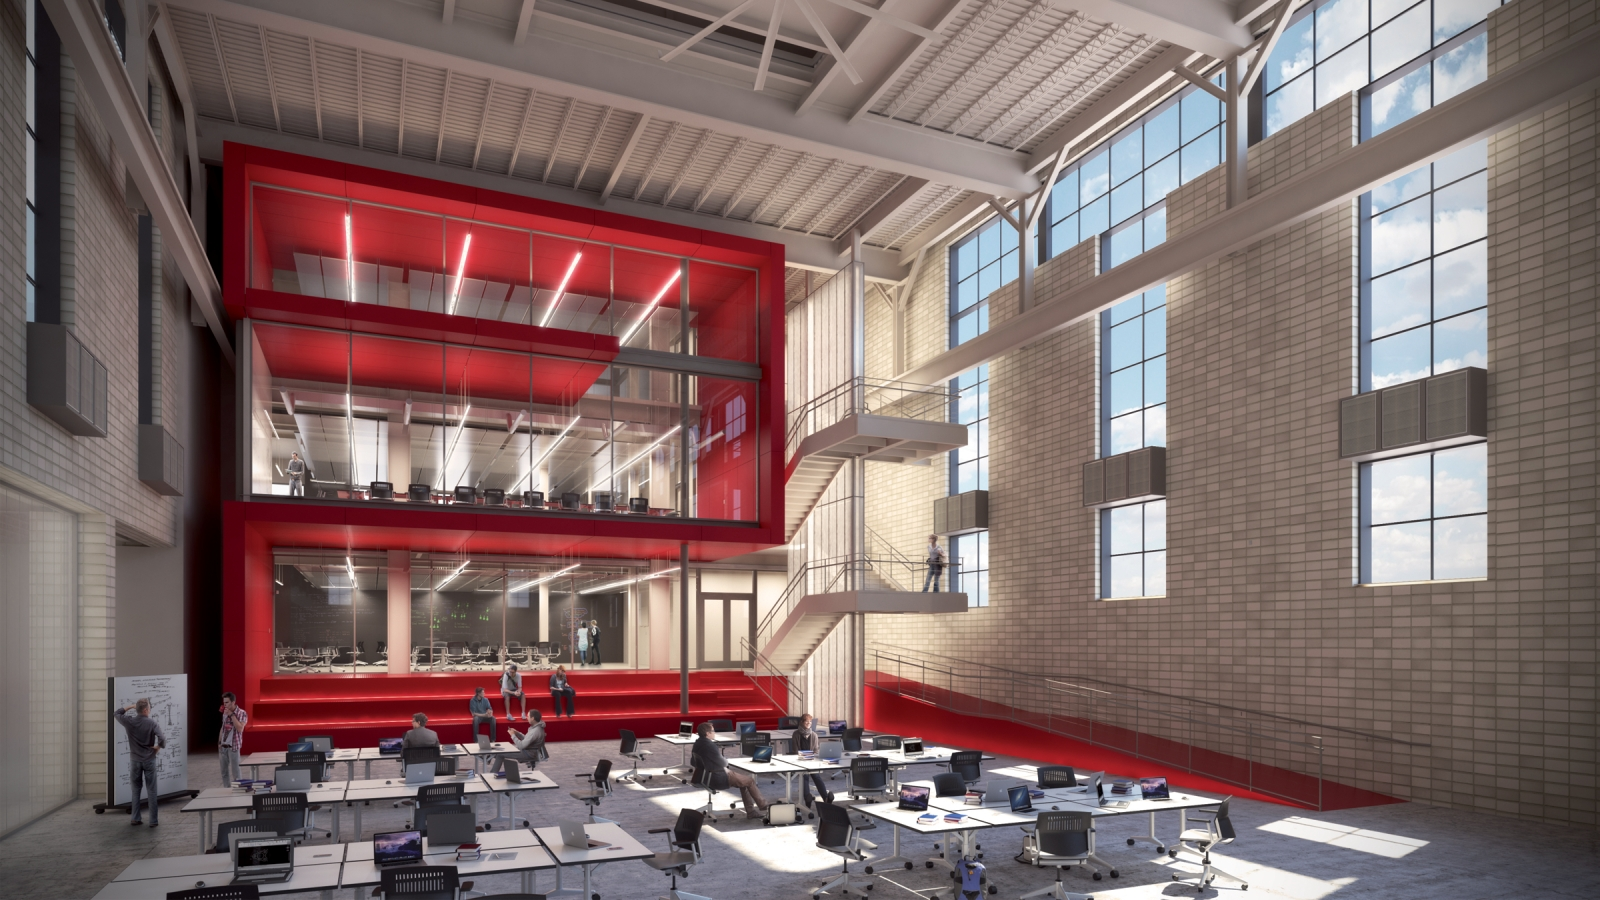
\includegraphics[height=3cm]{1012131_00_N5_bdc1_HERO.jpeg}
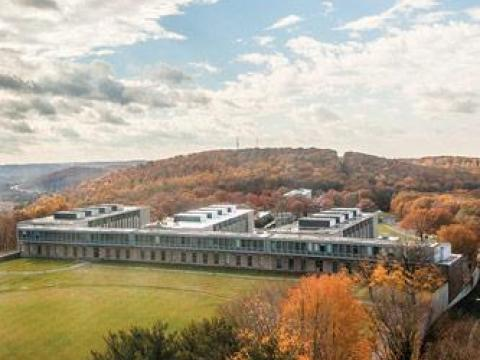
\includegraphics[height=3cm]{Mountaintop-BuildingC.jpg}
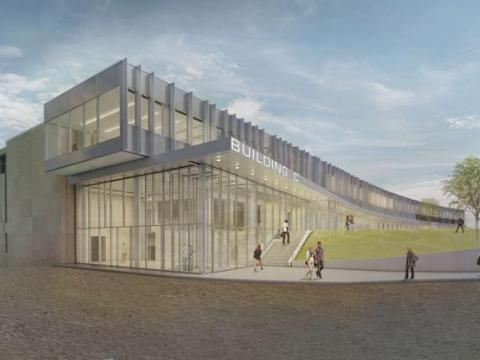
\includegraphics[height=3cm]{briefs-mountaintop-tech-building-initiative.jpg}
\end{center}
%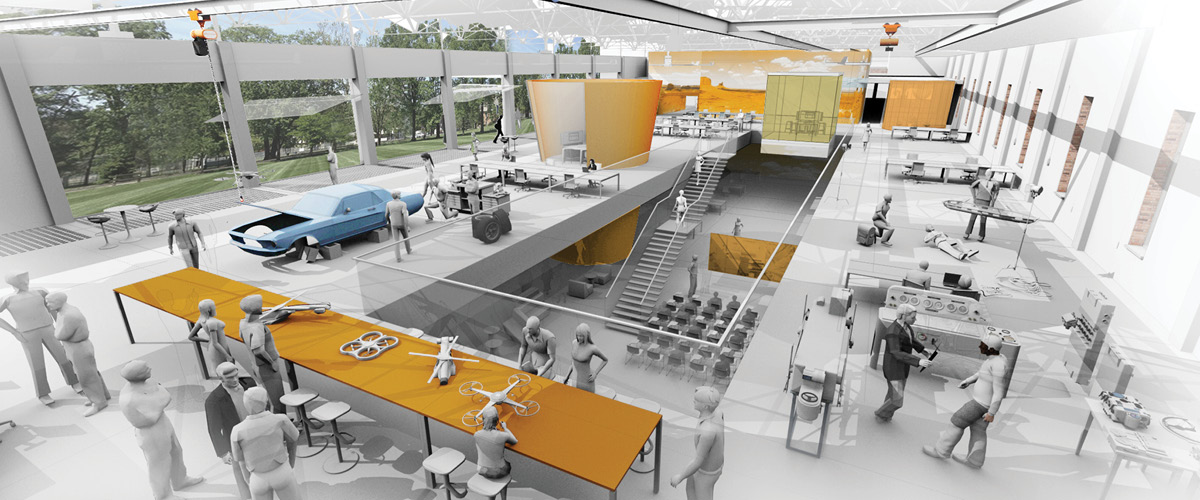
\includegraphics[height=3cm]{Path_to_Prominence_Lehigh_University_Evolution_MountaintopRendering_0.jpg}



\section*{Computing Resources}
  
\subsection*{Computing Resources at Lehigh University}
 
The Computational Optimization Research at Lehigh (\href{http://coral.ise.lehigh.edu}{COR@L}) Laboratory will be available for prototyping, benchmarking, and software development.  It has a cluster consisting of 15 CPU nodes, each with 16 cores and 32GB of RAM, as well as one GPU node with two nVidia K80 GPUs and 128GB of RAM.  The cluster has a variety of software tools for debugging and profiling.

To perform larger-scale testing, Lehigh University's central High Performance Computing (HPC) facilities will be utilized.  Lehigh's HPC facilities has a 
{\bf Sol cluster}, an 80-node HPC Cluster. 

 
\subsection*{Computing Resources at KAUST}
Dr.~Richt\'arik (collaborator for the project)
is keen to provide access to the KAUST super-computer {\bf Shaheen~II} (Cray XC40, Xeon E5-2698v3 16C 2.3GHz, Aries interconnect), currently the \href{https://www.top500.org/site/50205}{38th fastest super-computer} in the world to develop and test algorithms for training AI.
 

 

\section*{Partners for Broadening Participation}




\subsection*{Saucon Valley School District}
 
Saucon Valley school district is located 10 minutes drive from Lehigh. Robert Svitilla is high-school teacher and STEM coordinator in Saucon Valley High School.
 
 
 \begin{center}
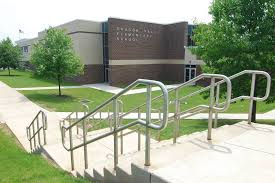
\includegraphics[height=3cm]{svsd.jpeg}
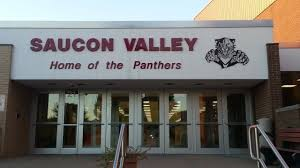
\includegraphics[height=3cm]{images.jpeg} 
\end{center}

\subsection*{Da Vinci Science Center}
The Da Vinci Science Center is located within a 20 minute drive from Lehigh.  Lehigh has well-established collaborations with the Da Vinci Science Center.

\begin{center}
\includegraphics[height=5cm]{Da_Vinci_Science_Center_05.jpeg}
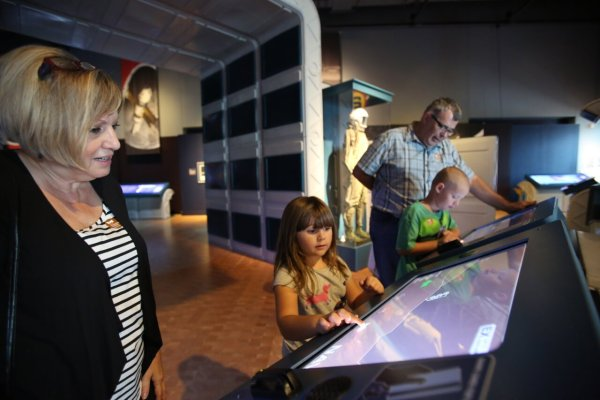
\includegraphics[height=5cm]{Be-the-Astro3.jpg}
\end{center}
 


\section*{Collaborators}   



\subsection*{Dr. Martin Jaggi, EPFL} 

\url{https://people.epfl.ch/martin.jaggi}\\
{\bf Short bio:}
Dr. Jaggi is a Tenure Track Assistant Professor at EPFL, heading the Machine Learning and Optimization Laboratory. His research interests lie in the fields of machine learning, optimization algorithms for learning systems, and text understanding. Before EPFL, he was a post-doctoral researcher at ETH Zurich, at the Simons Institute in Berkeley, US, and at École Polytechnique in Paris, France. He has earned his PhD in Machine Learning and Optimization from ETH Zurich in 2011, and a MSc in Mathematics also from ETH Zurich. He is a co-founder of the text analytics startup SpinningBytes, and also the founder of the Zurich Machine Learning and Data Science Meetup.

Dr. Jaggi will collaborate on developing efficient training algorithms for AI.

\subsection*{Dr. Alec Koppel, ARL} 

\url{https://koppel.netlify.com/}\\
{\bf Short bio:}
Dr. Koppel is a  Research Scientist with the U.S. Army Research Laboratory in the Computational and Information Sciences Directorate since September of 2017. His research focuses on optimization and machine learning methods for autonomous systems. He is currently pursuing works in:
Reinforcement Learning, 
Scalable online Bayesian and nonparametric methods.
Dr. Koppel has also worked on Online Learning and Stochastic Optimization;
Decentralized Optimization.

Dr. Koppel will collaborate on research related to "AI for Automated
Decision Making".
 
\subsection*{Dr. Peter Richt\'arik, KAUST; University of Edinburgh; Moscow Institute of Physics and Technology}
\url{https://richtarik.org}\\
{\bf Short bio:}
Dr. Richt\'arik is an Associate Professor of Computer Science and
Mathematics at the King Abdullah University of Science and Technology (KAUST). KAUST
is a new ``House of Wisdom,'' located on the shores of Red Sea in Saudi Arabia, modeled
after Caltech. He obtained his PhD from Cornell University in 2007, and have spent two years
immediately afterwards at the Centre for Operations Research and Econometrics, Universit\'e
Catholique de Louvain, as a CORE postdoctoral fellow, where he worked with Prof. Yurii
Nesterov. Since 2009, he held an Assistant (Lecturer) and later Associate (Reader) Professor
position appointments at the University of Edinburgh. At the moment he is also a Visiting
Professor at the Moscow Institute of Physics and Technology. He is  a Fellow of the Alan
Turing Institute---the UK national center for data science and artificial intelligence. His
work is mainly at the intersection of machine learning and optimization, with a focus on
training machine learning models using big data.


Dr. Richtarik will collaborate on research related to "AI with Limited Data in Physics" and "Data and Network Quantization".










\end{document}